\documentclass[
   12pt,                % Schriftgroesse 12pt
   a4paper,             % Layout fuer Din A4
   oneside,             % Layout fuer einseitigen Druck
   headinclude,         % Kopfzeile wird Seiten-Layouts mit beruecksichtigt
   %headsepline,         % horizontale Linie unter Kolumnentitel
   %plainheadsepline,    % horizontale Linie auch beim plain-Style
   BCOR12mm,            % Korrektur fuer die Bindung
   DIV18,               % DIV-Wert fuer die Erstellung des Satzspiegels, siehe scrguide
   halfparskip,         % Absatzabstand statt Absatzeinzug
   openany,             % Kapitel k�nnen auf geraden und ungeraden Seiten beginnen
   bibtotoc,            % Literaturverz. wird ins Inhaltsverzeichnis eingetragen
   pointlessnumbers,    % Kapitelnummern immer ohne Punkt
   tablecaptionabove,   % korrekte Abstaende bei TabellenUEBERschriften
   titlepage,			% ja bitte titelei
   nochapterprefix,
   appendixprefix,
   fleqn,               % fleqn: Glgen links (statt mittig)
   %draft               % Keine Bilder in der Anzeige, overfull hboxes werden angezeigt
     ]{scrartcl}

%\usepackage[onehalfspacing]{setspace}
\makeatletter
%\renewcommand*{\chapterheadstartvskip}{%
%	  {\setlength{\@tempdima}{\f@baselineskip}%
%	  \vspace*{2.3\@tempdima}}%
%	}
%\renewcommand*{\chapterheadendvskip}{%
%	  {\setlength{\@tempdima}{\f@baselineskip}%
%	    \vspace{1.725\@tempdima
%	      \@plus .115\@tempdima \@minus .192\@tempdima}}%
%	}
%\makeatother
%\usepackage{ngerman}             % neue Rechtschreibung
%\usepackage[ansinew]{inputenc}  % Input-Encodung: ansinew fuer Windows
\usepackage[latin1]{inputenc}    % Input-Encodung: latin1 fuer Unix
\usepackage[T1]{fontenc}         % T1-kodierte Schriften, korrekte Trennmuster fuer Worte mit Umlauten
%\usepackage{caption}      % mehrzeilige Captions ausrichten
\usepackage{url} 				 % fuer was auch immer
\usepackage[centertags]{amsmath} % AMS-Mathematik, centertags zentriert Nummer bei split
%\usepackage{latexsym}           % verschiedene Symbole
%\usepackage{textcomp}           % verschiedene Symbole
     
%\usepackage[pdftex]{graphicx}            % zum Einbinden von Grafiken
\usepackage{graphicx}            % zum Einbinden von Grafiken
\usepackage{float}               % u.a. genaue Plazierung von Gleitobjekten mit H

\usepackage{scrpage2}            % Kopf und Fusszeilen-Layout 
\renewcommand{\headfont}{\normalfont\sffamily}    % Kolumnentitel serifenlos
\renewcommand{\pnumfont}{\normalfont\sffamily}    % Seitennummern serifenlos
\pagestyle{scrheadings}

% kopfzeile - links mitte rechts
\ihead[]{Getting Started with DDT}              % Kolumnentitel immer oben innen
\chead[]{}
\ohead[\pagemark]{\pagemark}     % Seitennummern immer oben aussen
% fusszeile - links mitte rechts.
\ifoot[]{}
\cfoot[]{}
\ofoot[]{}                       % Seitennummern in der Fusszeile loeschen
\rohead{ 
\includegraphics[scale=0.5]{image/logo.pdf}}
\rofoot{\pagemark}
%\setheadwidth{textwithmarginpar}
%\setfootwidth{textwithmarginpar}
\newcommand{\titleRule}{\rule{\linewidth}{0.5mm}}


\reversemarginpar

% Schrift mit Serifen auch fuer Ueberschriften benutzen
%\renewcommand*{\sectfont}{\bfseries}
%\renewcommand*{\descfont}{\bfseries}

% define the wanted font for all highlightings here
\def\lstbasicfont{\fontfamily{pcr}\selectfont}

%% for sourcecode we use listings-package
\usepackage[usenames,dvipsnames]{color}
\usepackage{listings}
\definecolor{senacorlight}{rgb}{0.96,0.945,0.90} % original Senacor background color
\lstloadlanguages{Java}
\lstset{% general command to set parameter(s)+
basicstyle={\lstbasicfont\footnotesize},
%basicstyle={\ttfamily\small}, % print whole listing small
keywordstyle=\bfseries, % bold black keywords
basewidth=0.51em,
identifierstyle=\color{Black}, % gray
commentstyle=\color{Black}\itshape, % white comments
stringstyle=\color{Black}, % typewriter type for strings
showstringspaces=false, % no special string spaces
language=Java,
tabsize=2,
backgroundcolor=\color{senacorlight}
}

%\usepackage[intoc,german]{nomencl}
%\usepackage[german]{nomencl}
%\renewcommand{\nomname}{Glossar}
%\makenomenclature
%%% some defines

\typearea[current]{current}        % Neuberechnung des Satzspiegels mit alten Werten nach �nderung von Zeilenabstand,etc

%\usepackage{amsart}

\usepackage{ae}                  % F�r PDF-Erstellung
\usepackage{pdfsync}
\usepackage[pdftex,a4paper,
            pdftitle={Getting Started with DDT},
			pdfauthor={Hannes Leitl},
            colorlinks=false,
            bookmarks=true,
            bookmarksnumbered=true]{hyperref}



\begin{document}
\title{Getting Started\\with the Senacor DDT framework\\ \vskip 0.5cm 
\includegraphics[scale=0.5]{image/logo.pdf}}
%\author{Hannes Leitl}

\maketitle \tableofcontents
\thispagestyle{empty}


\section{Introduction} % (fold)
\label{sec:introductioin}

This is a short step by step tutorial that will teach you the basics of writing data driven tests with the Senacor \textsf{DDT} framework. All the examples included here may be downloaded from our subversion repository, so feel free to try them out and experiment further.


\subsection{Setting up your Java Environment} % (fold)
\label{sec:setting_things_up}

Your setup is easy. You'll need to be working with JDK version 1.4 (and up) with everything listed below in your class path.
\begin{itemize}
	\item \texttt{ddt-complete-}\emph{current$\_$version}\texttt{.jar} (if you downloaded the distribution version as a zip binary, this is one of the jars it contains. You may also use \texttt{ant} to build all \textsf{DDT}-jars from the sources. They will be created in the \texttt{build/jar} directory.)

	\item a bunch of third-party libraries from the \texttt{lib} directory: junit.jar, parallel-junit.jar, jxl-2.6.1.jar, commons-beanutils-core.jar, commons-logging.jar (- You could also just take everything you find under \texttt{lib})
	
	\item the directory where the Excel documents live: \\ \texttt{doc/tutorial/example$\_$src/com/senacor/ddt/tutorial}
	
\end{itemize}
% subsection setting_things_up (end)


\subsection{Choosing the Data Format} % (fold)
\label{sub:choosing_the_data_format}

The examples in this tutorial are set up for the use with MS Excel. Not because it is on our favorite product list but it is widely available in the enterprise world and well accepted. \textsf{DDT} supports other data formats but there is a reason why we think xls-support is the most important.

Just imagine you were able to show the quality of your piece of software by showing your customer a bunch of xls-files containing the data your tests will work with. They'll be happy campers because they feel home and cozy scrolling through even the biggest spread sheets. Although we feel much more comfortable with any plain text based format, our experience in enterprise projects leads us to the fact that customer acceptance is more important. They somehow \emph{trust} Excel so they will trust your tests even more when they are based on xls files. Just go with the flow.

% subsection choosing_the_data_format (end)
% section introduction (end)


\subsection{The Mission Critical Account Class} 

Most tutorials start off with a "hello world"--example but it's tough to come up with a meaningful test for that. So we chose the next boring example which came to our minds: A banking account class. It's perfectly fine for our little demonstration and the scenery isn't too unrealistic after all: Financial institutes are somewhat picky when it comes to software quality, so let's assume our customer is a bank and we want to make sure there are no bugs in the code we deliver.

So much for the big picture. Here is our bank account class called \emph{Account}. It couldn't be much simpler: An account has a balance and offers methods for making deposits and withdrawals. There is a small piece of logic for the situation when you wish to withdraw more money than you have. In that case it depends on whether you have a credit line or not: If not, only the remaining amount can be withdrawn. This is where a good unit test comes in handy.

\vskip 1em\begin{lstinputlisting}[frame=tb]{example_src/com/senacor/ddt/tutorial/Account.java}
\end{lstinputlisting}

What would be a good test? Let's think about a test scenario first before we get to the implementation. Using a spread sheet application we like (or Excel), we specify three different test cases which we think will cover all interesting aspects. Utilizing two different accounts, we transfer money from one account to another and  write down the expected values to be verified against. Take a look at the test sheet's screenshot in figure \ref{sheet1}.

\begin{figure}[H]
	\centering
	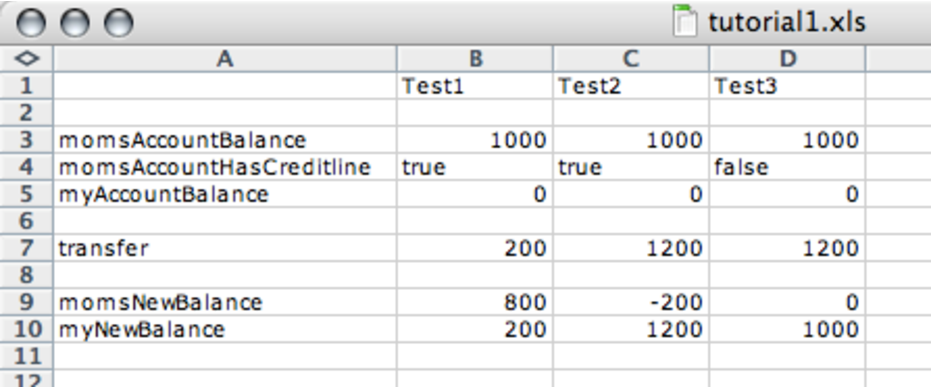
\includegraphics[scale=0.7]{image/sheet1.pdf}
	\caption{test cases for a money transfer}
	\label{sheet1}
\end{figure}


\section{A First Shot}\label{sub:my_first_ddt_test} % (fold)

Now that we know what the test cases will look like we need to read the data from the \texttt{xls} file into the test. The test class does not have to extend any special \textsf{DDT} base class, \texttt{AccountTest} is just a regular subclass of \texttt{junit.framework.TestCase}. It implements the \texttt{DataDrivenTestCase} instead which forces us to implement a getter and setter method for an instance of \texttt{TestCaseData}. All our data will be injected by the \textsf{DDT} framework into that instance as soon as we run the test.

\textsf{DDT} needs to know where to read the test data from. That aspect is handled by creating an \texttt{ExcelObjectMatrixFactory} which will be used by the \texttt{JUnitTestSuiteBuilder} to create a suite for you. For each column of the specified sheet of the given \texttt{xls}-file the test method will be run.

Please note that \textsf{DDT} expects the \texttt{xls}-file to be accessible from your class path.

\vskip 1em\begin{lstinputlisting}[frame=tb]{example_src/com/senacor/ddt/tutorial/AccountTest.java}
\end{lstinputlisting}

Once you start that test it will run all test methods once for each column of the spread sheet. Well, all columns but the first: It is used to name the lines of the matrix you refer to.
Take a look at the usages of \texttt{TestCaseData}'s \texttt{getBigDecimal}-method to retrieve a single value by the name that is written in the first column: \texttt{testCaseData.getBigDecimal("momsNewBalance")} will return an instance of \texttt{BigDecimal} for the value 200 in the first, -200 in the second and 0 in the third test case.

\texttt{TestCaseData} offers a bunch of getters for all common types. This is a good moment to go check its JavaDoc documentation to find out what is there for you to use.
% section my_first_ddt_test (end)


\section{Getting better}\label{sub:getting_better} % (fold)

In the last section you learned how to extract values from the sheet by using \texttt{TestCaseData}'s getter methods for each value. It is certainly nice to have \textsf{DDT} convert the text into the right types by using those convenient getter methods but it is still quite cumbersome to fill all of an object's properties that way. In our example, mom's account needs a balance to be set and the boolean value for the credit line. Now imagine that for an object with twenty attributes. It would clutter up your test source code.

\textsf{DDT} supports filling whole object graphs by letting you write paths instead of just names in the first column of the sheet. Technically we are saving only one line of code by using \texttt{TestCaseData}'s \texttt{fillBean} method to populate all properties at once instead of setting each value separately. For real world classes with lots of attributes and deep object graphs this is huge advantage, though. And there is another difference compared to the former version of the test class: You no longer have to worry about choosing the correct getter method to correspond the attribute's type. It is all handled by the \textsf{DDT} framework! 

\begin{figure}[H]
	\centering
	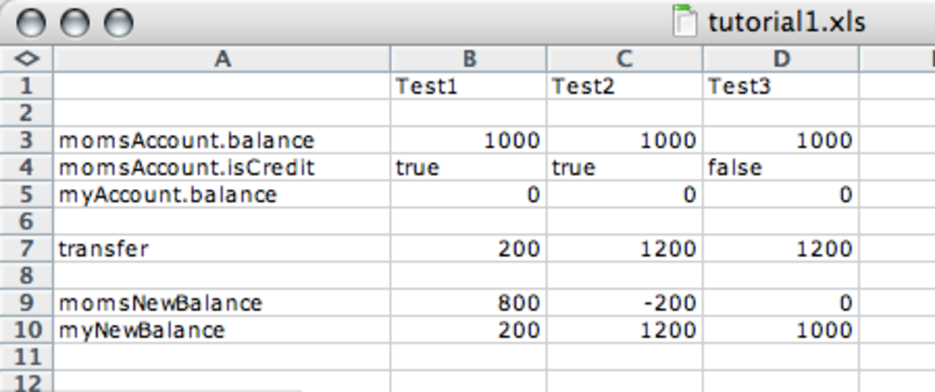
\includegraphics[scale=0.7]{image/sheet2.pdf}
	\caption{test cases for a money transfer}
	\label{sheet2}
\end{figure}


\vskip 1em\begin{lstinputlisting}[frame=tb]{example_src/com/senacor/ddt/tutorial/BetterAccountTest.java}
\end{lstinputlisting}
% section getting_clean (end)

\newpage

\section{An Almost Perfect Test Class} % (fold)
\label{sec:an_almost_perfect_test_class}
Now let's clean things up. In section \ref{sub:my_first_ddt_test} we filled the objects we need in our test from an Excel sheet but things still look kind of mixed up. To fix that we'll move all test case initializing code into the \texttt{setUp}-method so common objects may be used by additional test methods and leave \texttt{TestCaseData}-handling code in the test method only if it is specific to that test method. Take a look at the \texttt{testTransfer} method now: All that is left is pure test logic.

There is another improvement to our example test class. The name of the test cases are read from the test case sheet in the overridden \texttt{getName}-method so they can be displayed by the Junit runner as shown in figure \ref{testnames}. 

\begin{figure}[H]
	\centering
	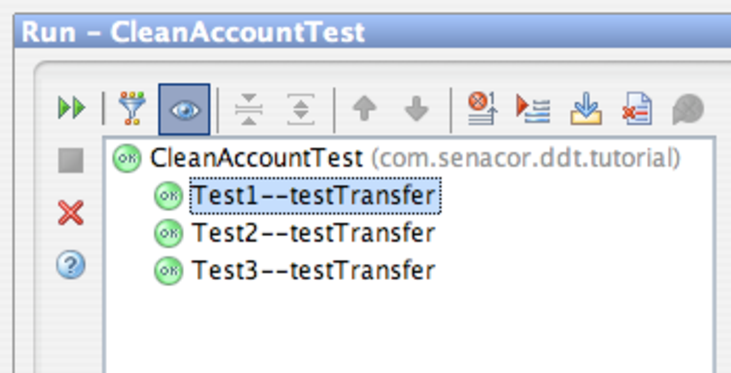
\includegraphics[scale=0.7]{image/testcasenames.pdf}
	\caption{test case names and test method names getting displayed}
	\label{testnames}
\end{figure}

\vskip 1em\begin{lstinputlisting}[frame=tb]{example_src/com/senacor/ddt/tutorial/CleanAccountTest.java}
\end{lstinputlisting}


% section an_almost_perfect_test_class (end)

\section{Advanced Stuff} % (fold)
\label{sec:advanced}

Now that you are familiar with the \textsf{DDT}'s basic features we are all set for our show off section. Take a look at the Excel sheet in figure \ref{sheet3}. That is what test data should look like, especially when we want to show that to our customer. \textsf{DDT} does not mind you using colors, text styles or data type specific cell formatting for readable calendar dates or currencies in monetary values. Note that we used "yes" and "no" instead of "true" and "false".\footnote{read all about \emph{transformers} in the technical documentation to learn how that works.}

This test proves that an account's balance will stay correct over time while some transfers will be processed at specific points of time. In the accounts section of the spread sheet two accounts will be set up. In the center block the transfers are specified and in the section titled "myBalances" the expected balances in certain points of time are stated.

\begin{figure}[H]
	\centering
	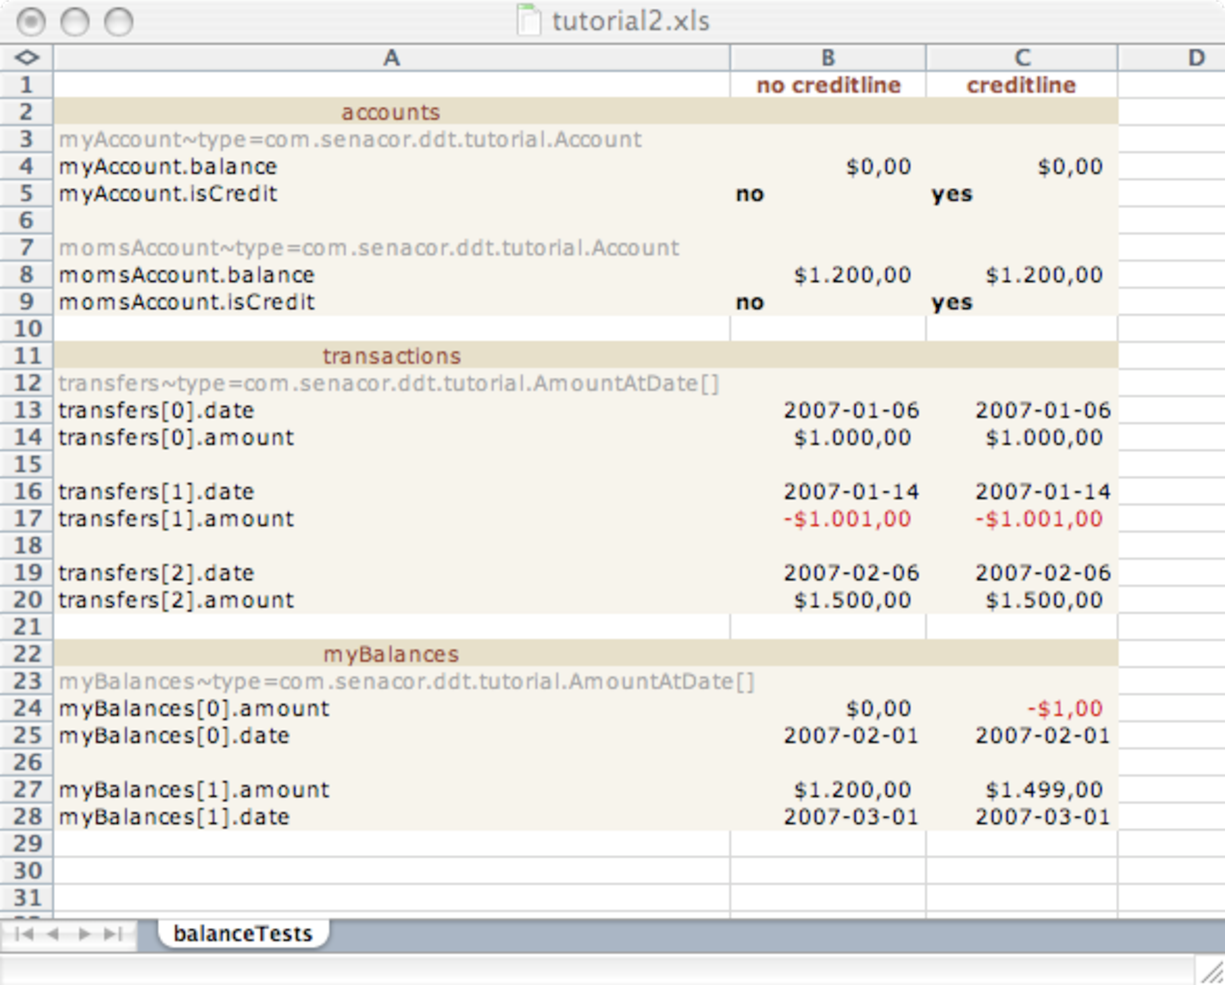
\includegraphics[scale=0.7]{image/advanced.pdf}
	\caption{an advanced sheet using formatting and expandable arrays}
	\label{sheet3}
\end{figure}

First of all, this example introduces a new class named \texttt{AmountAtDate} which is used as a container for the combination of a calendar date and an amount. It is common practice to create these kind of container classes to make extracting test case data easy.

\vskip 1em
\begin{lstinputlisting}[frame=tb]{example_src/com/senacor/ddt/tutorial/AmountAtDate.java}
\end{lstinputlisting}

The next thing you probably noticed is the use of brackets in the "transactions" and "myBalances" sections. That notation is used to describe elements of an array, just like you would write the same in Java source code. Here comes the real big deal with that feature: Without changing the code of your test class you are able to expand your test case by adding new array elements. Just add some lines and increment the index. \textsf{DDT} will expand the array for you as it reads in the additional line. That means your customer may not only create new test cases by adding new columns to the sheet but also by adding new lines for array elements that will be automatically read when running the test. Let the business folks deliver the contents as you provide the logic of the test class!

Take a look at the test code that imports the data from the sheet: The method \texttt{testBalances} reads two arrays from the test sheet but it does not instantiate the arrays by itself. \textsf{DDT} even creates the array for you when you call \texttt{TestCaseData}'s \texttt{createAndFillBean}-method. But how does it know what type of bean (or array in this case) need to be used? That's what the type annotation\footnote{\textsf{DDT}-annotations start with the tilde sign} in the spread sheet is for. By placing the line 
\begin{lstlisting}[]{}
	transfers~type=com.senacor.ddt.tutorial.AmountAtDate[]
\end{lstlisting} 
you tell \textsf{DDT} that it has to create an array of type \texttt{AmountAtDate}, whereas
\begin{lstlisting}[]{}
	myAccount~type=com.senacor.ddt.tutorial.Account
\end{lstlisting} denotes an instance of class \texttt{AmountAtDate}.

The ability to create objects not just fill existing objects with data during the spread sheet import is important for two things: If you want to be type safe you need to work with arrays instead of collections but arrays need to be sized correctly when instantiated. Since you don't know how many entries an array will get there is no way of creating the array in advance. \textsf{DDT} resizes arrays as necessary while reading the spread sheet. Furthermore, all entries of an array must not be instances of the same class when using inheritance. You could denote the first entry of transfers to be an instance of \texttt{MySpecialAmountAtDate} (that has to extend \texttt{AmountAtDate}) by inserting
\begin{lstlisting}[]{}
	transfers[0]~type=com.senacor.ddt.tutorial.MySpecialAmountAtDate
\end{lstlisting} 
assuming \texttt{MySpecialAmountAtDate} extends \texttt{AmountAtDate}.

\vskip 1em
\begin{lstinputlisting}[frame=tb]{example_src/com/senacor/ddt/tutorial/BalanceTest.java}
\end{lstinputlisting}

% section advanced (end)

\section{Where to Go from Here} % (fold)
\label{sec:where_to_go_from_here}

Now that you got things started, you will probably want to have a look at the \textsf{DDT Reference Manual} which offers an architectural overview and plenty of detailed information about how to get the most out \textsf{DDT}.

You might also want to check \texttt{http://ddt.senacor.com} for recent news about this project.

% section where_to_go_from_here (end)

\end{document}